\chapter{Introduction}
\section{Background}
Cloud computing has undergone a significant transformation, especially for businesses, allowing them to create scalable, on-demand resources and easily accessible distributed systems for their applications.
Services like accessing finances, accessing health, running powerplants, managing traffic, and managing public resources are a few examples of where cloud technologies are in use \citep{intro_cloud_critical_infra}.
This transformation is fundamentally changing the traditional methods of self-hosting infrastructure and replacing them with continual innovations, enhancing efficiency and improving user experience by providing a digital platform in the form of different applications/software hosted in the cloud.
For example, in 2023, the German administration created a cloud strategy plan with the German Administration Cloud Strategy (DVS) to incorporate, strengthen and improve the status quo of digitalisation in the public sector \citep{german_gov_cloud_plan}.
Such policies are not isolated to a single country and signal a move towards cloud and digitalisation to shape the new world. \newline

As this modernization reshapes the business landscape, there is a need to ensure that only legitimate users gain access to sensitive data.
Systems need to protect personal data, and unauthorised breaches, to prevent loss of intellectual property, violation of laws and regulations and disruption to public services \citep{critical_infra_reason}.
Therefore, \textit{authentication} and \textit{authorisation} are fundamental concepts in cybersecurity, crucial for safeguarding digital resources and ensuring proper access control.
\newline
Authentication is the process of verifying the identity of a user or an application using credentials like passwords, biometrics, or tokens \citep{authetication_intro}.
On the other hand, authorisation determines the permissions or defines the granular access levels a user can execute, ensuring only the actions one is entitled to are used \citep{Gollmann2021-at}.
Having both mechanisms to secure systems and avoid the leakage of sensitive information and unauthorised access is especially important as cloud computing becomes more prevalent.
Many services are easily accessible to a larger group of people, as running and creating different applications is easier, which simultaneously gives attackers more systems to compromise.\newline

In addition to the benefits that cloud computing provides, such as easy accessibility and quicker setup of applications, it has also introduced new challenges.
In particular, the shared responsibility model of the cloud, where the cloud provider and the client both have specific responsibilities to secure the system \citep{shared_principal}.
The shared responsibility model means that any misconfiguration or oversight on either side could leave the system vulnerable to attack.
For instance, if the cloud provider maintains a secure infrastructure but the client misconfigures their application or leaves private databases open to the public, this could lead to data breaches or exploitation.
This complication increases exploitable attack surfaces as different errors and misconfiguration could make the system more vulnerable.
Therefore, integrating authentication and authorisation mechanisms for cloud-based applications has become increasingly vital.
These processes ensure that sensitive information is protected and access is restricted solely to authorised entities who require it. \newpage


\section{Problem Statement}
Although cloud computing offers easy scalability, on-demand distributed system access and efficiency to its consumers, it presents significant security challenges, such as \textit{authentication} and \textit{authorisation}.
Vulnerabilities in this area can lead to unauthorised access and data breaches, which are costly.
In 2023 the average cost of a data breach is 4.45 million USD  \citep{statista_data_breach}.
Given its widespread adoption of cloud and the OpenID Connect, this thesis investigates the security risks of authentication and authorisation in cloud-based applications using the OIDC protocol, a leading framework for Identity Management (IdM) supporting use cases such as mobile applications, machine-to-machine communication, and Single Sign-On (SSO)  \citep{oidc_popular}.


\section{Research Question}\label{sec:objectives}
The motivating research questions for this work can be stated as follows: \newline
\textbf{\textit{RQ1: What are the primary security concerns of the OpenID Connect protocol when used in a cloud-based application?}.} \newline 
Alongside the primary research question, a secondary research question is also taken into account, which is: \newline
\textbf{\textit{RQ2: What are the mitigation strategies that can be implemented for the risks identified?}.} 

\section{Aims and Objectives}
The primary aim of the RQ1 is to systematically analyse the security risks associated with implementing and using the OIDC protocol in cloud-based applications by identifying common vulnerabilities, assessing their impact on the overall security of these applications, and proposing effective mitigation strategies.
Pursuing this aim, the thesis has the following objectives and goals:

\begin{enumerate}
  \item Identify Common Security Risks - 
  \begin{itemize}
      \item Evaluate at least five security risks for the cloud and five for OIDC protocol and describe their effects.
      \item Evaluate security risks only from research dating from 2020 to 2024.
  \end{itemize}

    
  \item Conduct Risk Assessment  - 
  \begin{itemize}
      \item Implement STRIDE threat modelling for the evaluated risks.
      \item Propose specific mitigation strategies for each identified threat.
      \item Create a risk matrix with probability and impact scores.
      \item Assess non-compliance risks for privacy law like the General Data Protection Regulation. 
  \end{itemize}
  \item Prototype Development and Validation - 
  \begin{itemize}
      \item Develop a working proof-of-concept incorporating identified security controls in a simulated cloud environment.
      \item Implement at least five of the identified mitigation strategies in the prototype.
      \item Achieve a minimum of 90\% code coverage in unit testing.
      \item Perform Manual and automated testing for the security controls implemented.
  \end{itemize}
\end{enumerate}

\section{Research Methodology}
The research adheres to the Design Science Research Methodology (DSRM) for Information Systems Research.

The DSRM is a robust framework for studying, creating, and evaluating IT artefacts.
It is a suitable choice for this master thesis, which aims to design and develop artefacts for the OIDC protocol in a cloud-based application.
This methodology is favoured because it provides specific guidelines for creating and implementing information systems \citep{dsrm}.

The DSRM framework encompasses six steps: problem identification, definition of objectives, design and development, evaluation, demonstration, and communication \citep{dsrm}.
Figure \ref{fig:dsrm} depicts the six steps mentioned and how they would be used in this project and describes the implementation of this framework.
These steps align seamlessly with the goals of this research.
The primary aim of this project is to identify and evaluate potential risks associated with the OIDC protocol in a cloud-based application.
Based on the insights gained from this evaluation, the project proceeds to design, create, and rigorously test a prototype.
This approach ensures a structured and methodical examination of the OIDC protocol’s vulnerabilities and mitigations, thus aligning with the objectives outlined in section \ref{sec:objectives}.

In detail, the DSRM process begins with problem identification, where the specific security challenges and vulnerabilities of the OIDC protocol in cloud environments are identified.
Following this, the objectives are defined, and clear goals for the research are set, particularly regarding risk assessment and artefact development.
The design and development phase involves creating security artefacts, such as threat models based on the discovered risks.

The evaluation phase will assess these artefacts through various code and security testing methods to ensure their effectiveness and reliability.
Demonstration involves showcasing the developed prototypes in practical scenarios to validate their functionality.
Finally, the communication phase focuses on disseminating the findings and methodologies through comprehensive documentation and presentations, ensuring that the research contributes valuable insights to the broader field of information systems security.

By adhering to this structured methodology, this work addresses the immediate goals of evaluating and mitigating risks associated with the OIDC.
It provides a qualitative analysis that can inform future developments in the field.
DSRM ensures that each research phase is meticulously planned and executed, ultimately leading to the development of robust security solutions for this use case.

\begin{figure}[h!]
\centering

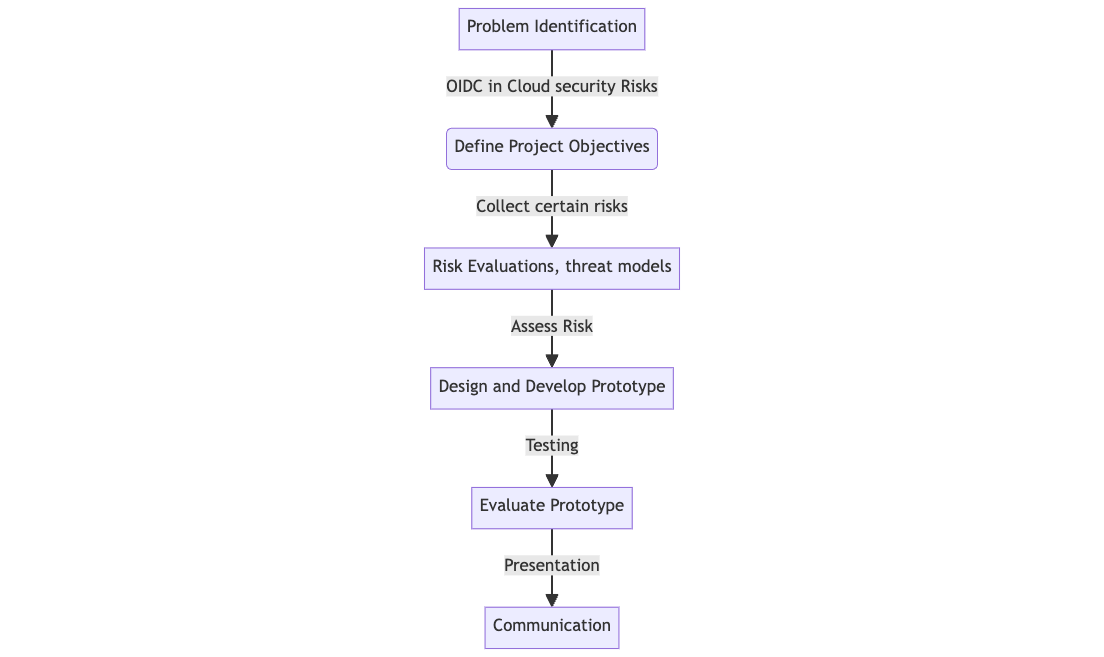
\includegraphics[width=\textwidth, height=350px]{pics/dsrm.png}
\caption{DSRM Methodology}
\label{fig:dsrm}
\end{figure}
\newpage
\section{Thesis Outline}

This master's thesis project outlines six chapters:

\begin{itemize}
    \item \textbf{Chapter 1} - In the introduction chapter, we will explore the background of cloud applications and the implementation of OpenID Connect. This examination will include a definition of a specific problem statement that addresses the security challenges associated with these technologies. Following this, we will outline the research methodology and approach that will be utilised to investigate the identified issues. 
    

    \item \textbf{Chapter 2} - This chapter analyses existing work from research papers, journals, documentation, books, conference papers, theses and other scholarly sources concerning cloud application and OIDC.
    In addition to analysing and summarising the theories, a discussion identifies gaps in the existing literature for the applications using OIDC in the cloud environment. Finally, identifying research gaps is vital for fostering innovation and ensuring that future studies address real-world needs in cloud security and application development.
    
    \item \textbf{Chapter 3} - In this chapter, we identify common attack vectors for OIDC and cloud environments and develop a comprehensive threat model using the STRIDE method. Additionally, conduct a risk assessment analysis and propose mitigations for the risks identified during the assessment.
    
    \item \textbf{Chapter 4} - In this chapter, we select a suitable cloud provider and outline the system architecture tailored to the project. Implement and design security controls to safeguard the system. Finally, document the methodology used for setting up the prototype and implement the application in the cloud environment.
    
    \item \textbf{Chapter 5} - This chapter presents the results from the developed prototype. We will conduct various checks to prove the effectiveness of the implementation. These tests include manual tests as well as automated test results. The results from these tests are carefully analysed and documented. Finally, the findings are presented to stakeholders for review.
    
    \item \textbf{Chapter 6} - This chapter is the final section of this report, where the conclusions from the investigations and the future work that can be done to this research are presented. Future research directions should explore unresolved questions and expand on the established findings to deepen knowledge in the field.

\end{itemize}